\documentclass[%
a4paper,
%twoside,
11pt
]{article} 

% encoding, font, language
\usepackage[T1]{fontenc}
\usepackage[latin1]{inputenc}
\usepackage{lmodern}
\usepackage[ngerman]{babel}
\usepackage{graphicx}
\usepackage{nicefrac}


\usepackage[
    nowarnings,
    %myconfig 
]
{xcookybooky}
 

\DeclareRobustCommand{\textcelcius}{\ensuremath{^{\circ}\mathrm{C}}}


\setcounter{secnumdepth}{1}
\renewcommand*{\recipesection}[2][]
{%
    \subsection[#1]{#2}
}
\renewcommand{\subsectionmark}[1]
{% no implementation to display the section name instead
}
%\setRecipeColors{recipename=blue}

\usepackage{hyperref}    % must be the last package
\hypersetup{%
%    pdfauthor            = {Sven Harder},
    pdftitle             = {Mamas Kochbuch},
    pdfsubject           = {Recipes},
    pdfkeywords          = {example, recipes, cookbook, xcookybooky},
    pdfstartview         = {FitV},
    pdfview              = {FitH},
    pdfpagemode          = {UseNone}, % Options; UseNone, UseOutlines
    bookmarksopen        = {true},
    pdfpagetransition    = {Glitter},
    colorlinks           = {true},
    linkcolor            = {black},
    urlcolor             = {blue},
    citecolor            = {black},
    filecolor            = {black},
}

\hbadness=10000 % Ignore underfull boxes

\begin{document}

\title{Mamas Kochbuch}

\maketitle

\setHeadlines
{% translation
    inghead = Zutaten,
    prephead = Zubereitung,
    hinthead = Tipp,
    continuationhead = Fortsetzung,
    continuationfoot = Fortsetzung auf n\"achster Seite,
    portionvalue = Personen,
}


\tableofcontents

\vspace{5em}
\newpage
\section{Kuchen}

\begin{center}
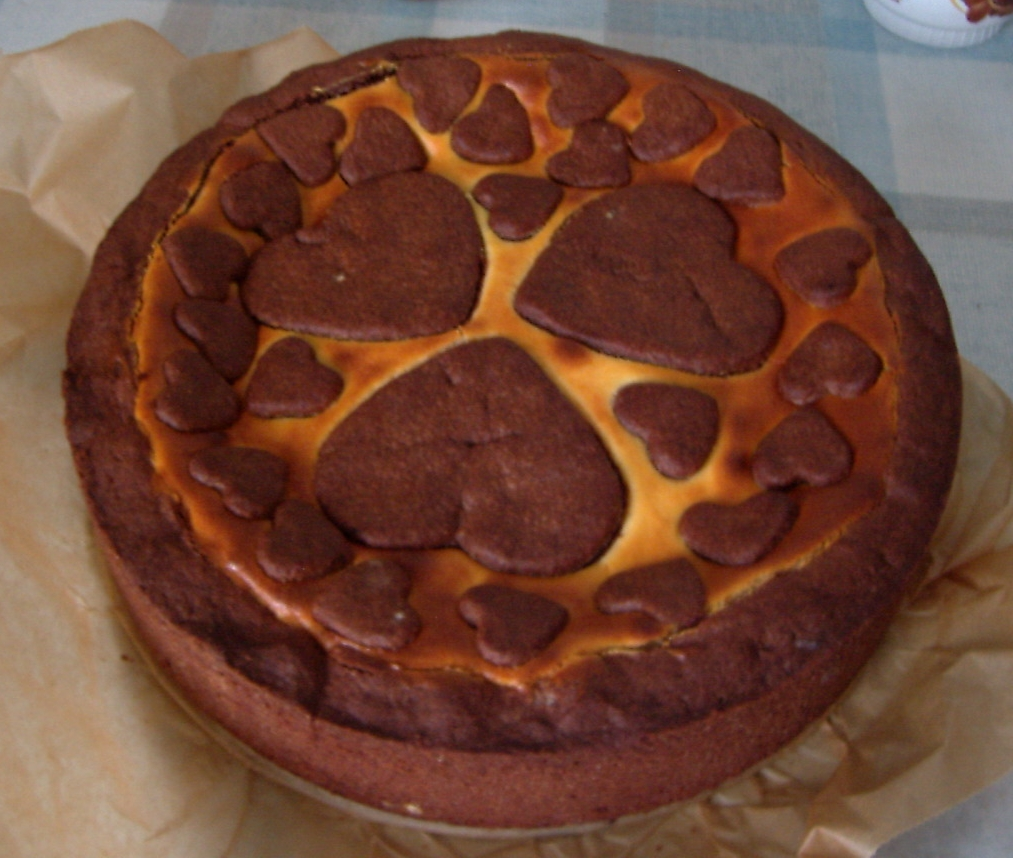
\includegraphics[width=0.8\textwidth]{./Bilder/RussischerZupfkuchen}
\end{center}


\newpage

\begin{recipe}
[ % Optionale Eingaben
    bakingtime={\unit[30]{min}},
    bakingtemperature={\unit[200]{\textcelcius}},
%    portion = {\portion{5-6}}
]
{Donauwellen}
    
    \graph
    {% Bilder
%        small=glass,    % kleines Bild
        big=./Bilder/Donauwellen % gro�es (l�ngeres) Bild
    }
    
    \ingredients
    {% Zutaten
	    \unit[250]{g} & Butter \\
		\unit[350]{g} & Mehl \\
		6 & Eier\\
		\unit[200]{g} & Zucker\\
		\unit[1]{Pck.} & Vanillezucker \\
		\unit[1/2]{Pck.} & Backpulver \\
		2 Gl�ser & Sauerkirschen\\
		\unit[2]{EL} & Kakao\\
		\ \\
		\unit[1]{Pck.} & Paradiescreme Vanille \\
		\unit[400]{ml} & Schlagsahne \\
		\ \\
		\unit[1-2]{Pck.}& Schokoglasur \\
    }
    
        
    
    
    \preparation
    { % Zubereitung
        \step Butter schaumig r�hren. Nach und Nach Zucker und Eier zugeben. Mehl und Backpulver mischen und essl�ffelweise zugeben.
        \step Etwa die H�lfte des Teiges auf das Backblech streichen. Den restlichen Teig mit dem Kakao verr�hren und auf dem hellen Teig verteilen.
        \step Mit einer Gabel Wellen im Teig ziehen. Die abgetropften Kirschen auf dem Teig verteilen. Bei \unit[200]{\textcelcius} f�r \unit[30]{min} backen.
        \step Die Paradiescreme mit der Sahne f�r ungef�hr \unit[3]{min} mit dem Handr�hrger�t schlagen und auf dem erkalteten Kuchen verteilen. Mit der Schokoglasur verzieren.
    }
    
    \hint
    {% Tipp
        Eine Portion Paradiescreme ist wenig, zwei sind viel.
    }

\end{recipe}

%\newpage

\end{document} 